\documentclass{article}
% Load packages
\usepackage{tikz} % to draw neural network
\usepackage{lscape}
\usepackage{graphicx}   % Including figure files
\thispagestyle{empty}
\begin{document}
%\begin{landscape}
%\begin{figure}
%    \centering
%    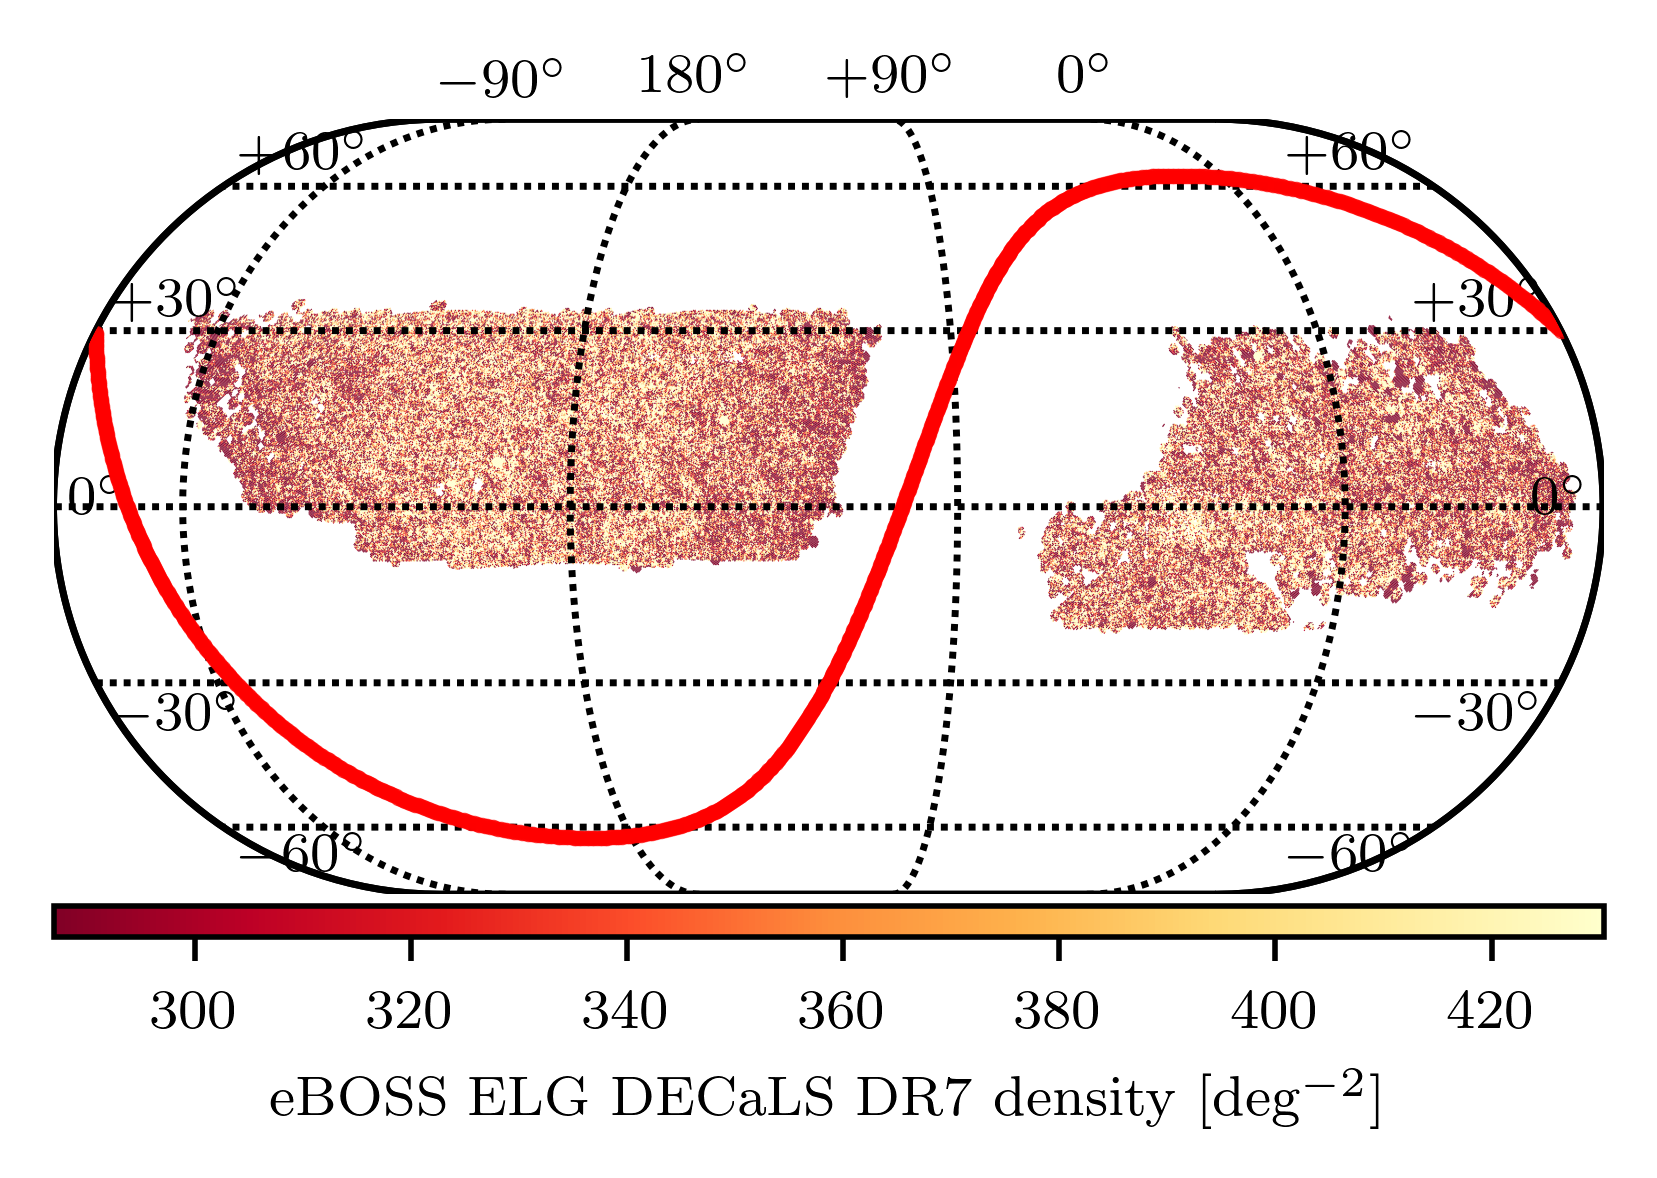
\includegraphics[width=\textwidth]{eboss-dr7.png}
%    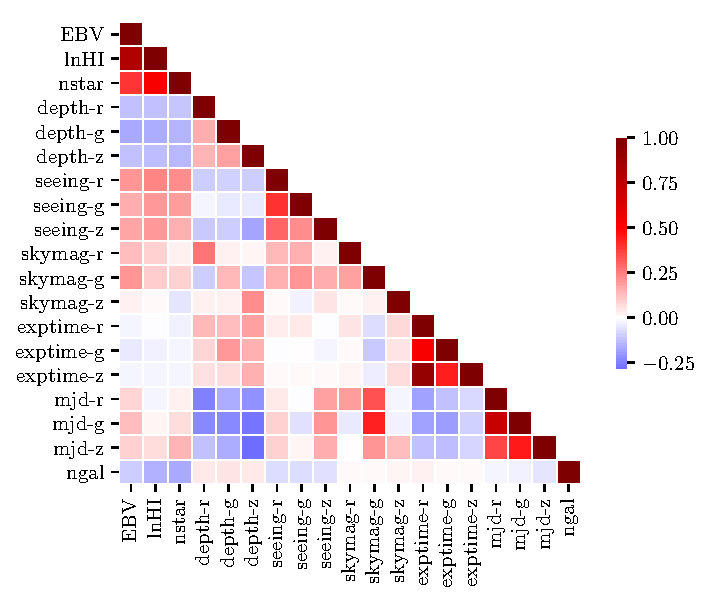
\includegraphics[width=\textwidth]{corrmax-dr7.pdf}
%\end{figure}
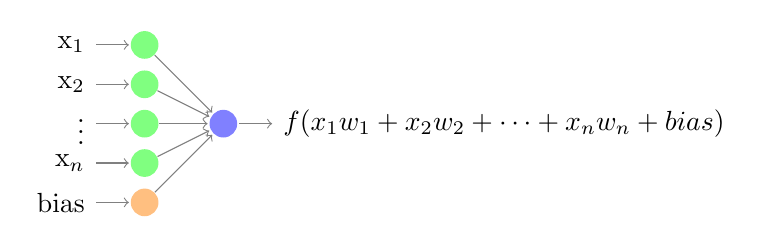
\begin{tikzpicture}[shorten >=0.5pt,->,draw=black!50, node distance=1.cm]
    \tikzstyle{every pin edge}=[<-,shorten <=0.5pt]
    \tikzstyle{neuron}=[circle,fill=black!25,minimum size=10pt,inner sep=0pt]
    \tikzstyle{input neuron}=[neuron, fill=green!50];
    \tikzstyle{hidden neuron}=[neuron, fill=blue!50];
    \tikzstyle{bias neuron}=[neuron, fill=orange!50];
    % Draw the input layer nodes
    \foreach \name / \y in {x$_{1}$/3, x$_{2}$/4, \vdots/5, x$_{n}$/6}
        \node[input neuron, pin=left:\name] (I-\y) at (1. cm,-0.5*\y cm) {};            
    \node[bias neuron, pin=left:bias] (I-7) at (1. cm,-3.5) {};          
     % Draw the output layer node
    \node[hidden neuron,pin={[pin edge={->}]right:$f(x_{1}w_{1} + x_{2}w_{2}+ \cdots + x_{n}w_{n}+ bias)$}, right of=I-5] (O) {};
    \foreach \source in {3,...,7}
        \path (I-\source) edge (O);
\end{tikzpicture}
%\end{landscape}
\end{document}

